\section{Dataset}
\subsection{Data Scale}
%介绍数据集的大致情况

%给一个sample
With the hierarchical structure as audios, sentences, words and syllables, 
we have given each of the barks of Shiba Inu dogs symbolic transcripts. 
The distributions of each tier are shown in~\tabref{tab:datasetinformation}. As the whole videos are got from open public media YouTube, they contain a large excess of non-labeling fragments, when the dog doesn't bark or some noise such as human speech and background music. What we concern more are those barking fragments, that is the ``sentences.'' We can take the length of sentences as the length of our dataset. At the same time, because we obtain our data from YouTube, the dataset size can grow over time with more users uploading videos.
% \KZ{Give the length in terms of minutes, instead of seconds? And we need to argue that the dataset can grow over time.}


%时长,句平均时长,句时长方差,词平均时长,词时长方差,平均句含词数量$
\begin{table}[th]
\centering
\small
\begin{tabular}{c|c|c|c|c}
\hline
\multirow{2}{*}{\textbf{DogID}} & \multicolumn{2}{c|}{\textbf{Sentence}} & \multicolumn{2}{c}{\textbf{Word}}  \\
\cline{2-5}
{} & \textbf{Num} & \textbf{Duration (s)} & \textbf{Num} & \textbf{Duration (s)} \\
\cline{1-5}
0 & 40 & 135 & 65 & 27 \\ %7 shibainu_rikuchannel
1 & 52 & 157 & 77 & 47\\ %6 ringoro
2 &  55 & 171 & 123 & 65\\ %3 hikaiti
3 &  56 & 224 & 107 & 94\\ % 4 jumpingmameko1822
4 & 87 & 299 & 134 & 101 \\ %15 shibaneko
5 & 118 & 350 & 324 & 144\\%14 shibainutakanoriawesomecha30
6 &  115 & 374 & 217 & 98\\ %5 MomoTenKuu
7 & 158 & 514 & 241 & 129\\%1 mamedachamesuke
8 & 130 & 562 & 257 & 147\\ %12 ShibainuRanmaru
9 &  135 & 566 & 316 & 143\\ %8 shibainu-rara
10 & 188 & 570 & 320 & 203\\ %11 ShibainuKOTETSU
11 & 255 & 795 & 408 & 157\\%9 shibainucatchannel7691
12 & 346 & 1107 & 577 & 363\\ %0  mamedachamesuke
13 &  553 & 1643 & 847 & 469\\%2 user-kd8rn5jx7x
14 & 993 & 2930 & 1719 & 749\\%13 shibainuTAIGA
15 & 1188 & 4306 & 2029 & 1372\\%10 ShibaInuKohachannel
\cline{1-5}
avg. & \textbf{279} & \textbf{919} & 485 & 269\\\hline
\end{tabular}
\caption{The basic statistical information of ShibaScript.}
\label{tab:datasetinformation}
\end{table}



\subsection{Data Variety}
%scene and acitivity show,展示我们的数据集cover了一个很大范围的scene & activity

% 总述,讲范围大
Shiba Inu is a very common and lively breed of dog, many people like them and keep them as pets. Those hosts live with their dogs and record their daily lives through videos. As the dataset ShibaScipt is transcribed from the audios extracted from life recording videos on YouTube, the dogs may appear in a variety of common and even uncommon scenes rather than a limited set of scenes, and they may be doing many activities. Therefore, ShibaScript covers a very diverse set of scenes and activities, including 37 different scenes and 44 different activities for dogs. What's more, unlike other datasets which record audios in fixed scenes or manually, the scenes and activities covered by ShibaScript can be expanded as the dataset is continuously collected.

% 多样性, 常见的场景和活动在大部分用户的视频中都出现,突出大数量的优点
~\figref{fig:scene_and_activity} shows the scenes and activities covered by ShibaScript. We can find that there is a subset of the activities that appear in the vast majority of users' videos. For pet dogs, their daily activities such as walking, running, and sleeping are essential and common, and their owners may also record these activities, so these daily activities are covered by most of the users. This holds for the statistical results of scenes as well, that common scenes in daily life like ``quilt'', ``road'', ``bedroom'', ``dog bowl'' appear in the vast majority of users' videos. Benefiting from the large number of videos used to transcribe the dataset, ShibaScript covers the vast majority of everyday scenes and activities.

% \KZ{You should use subfig here properly. Then
% you can make these two figs slightly bigger.}
\begin{figure}[ht]
\scalebox{0.37}{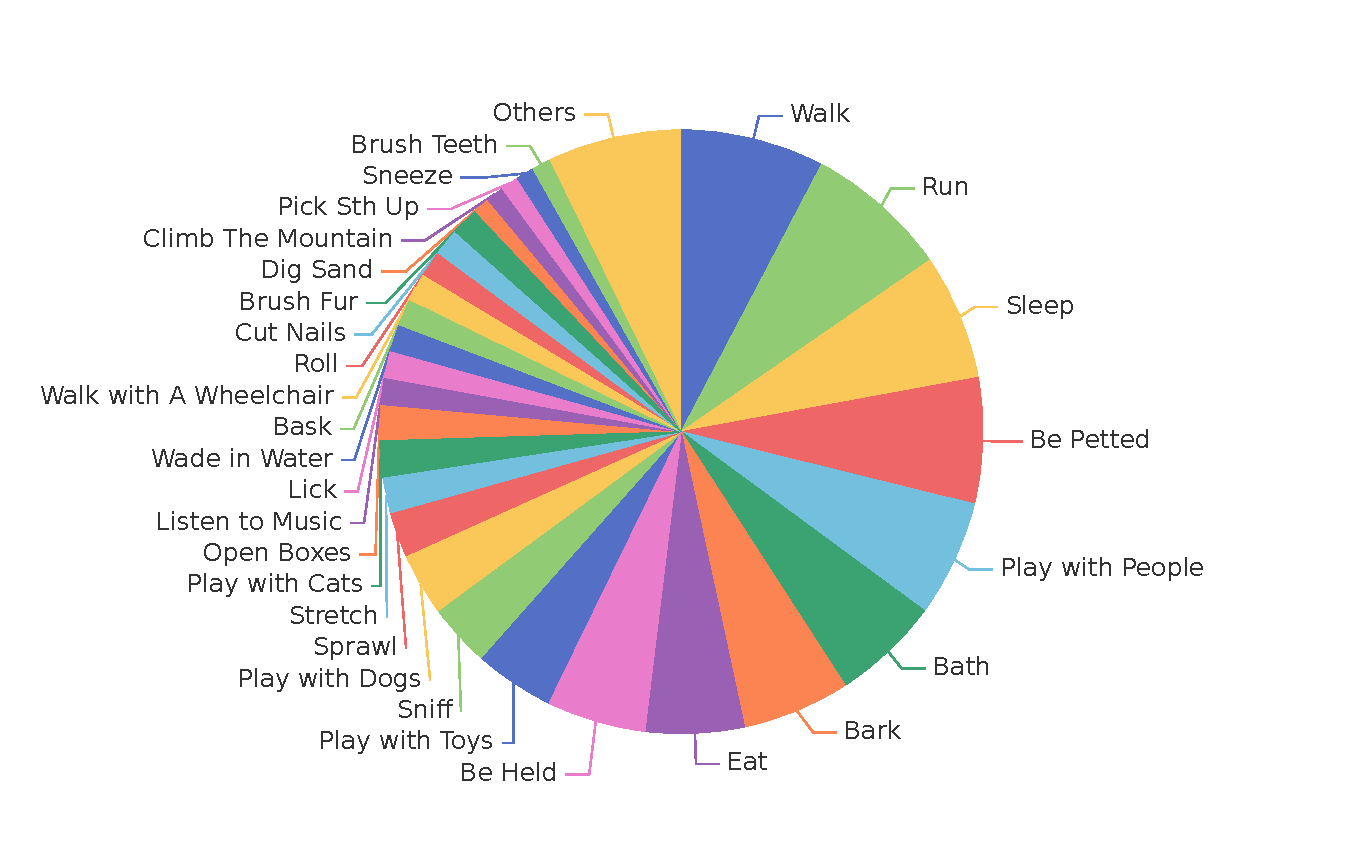
\includegraphics{total_activities.pdf}}
(a) Activities covered by ShibaScript. The activities which occurrences is less than 5 were merged into ``others'', see~\secref{sec:appendix_a} for details.~\\
\\
\scalebox{0.37}{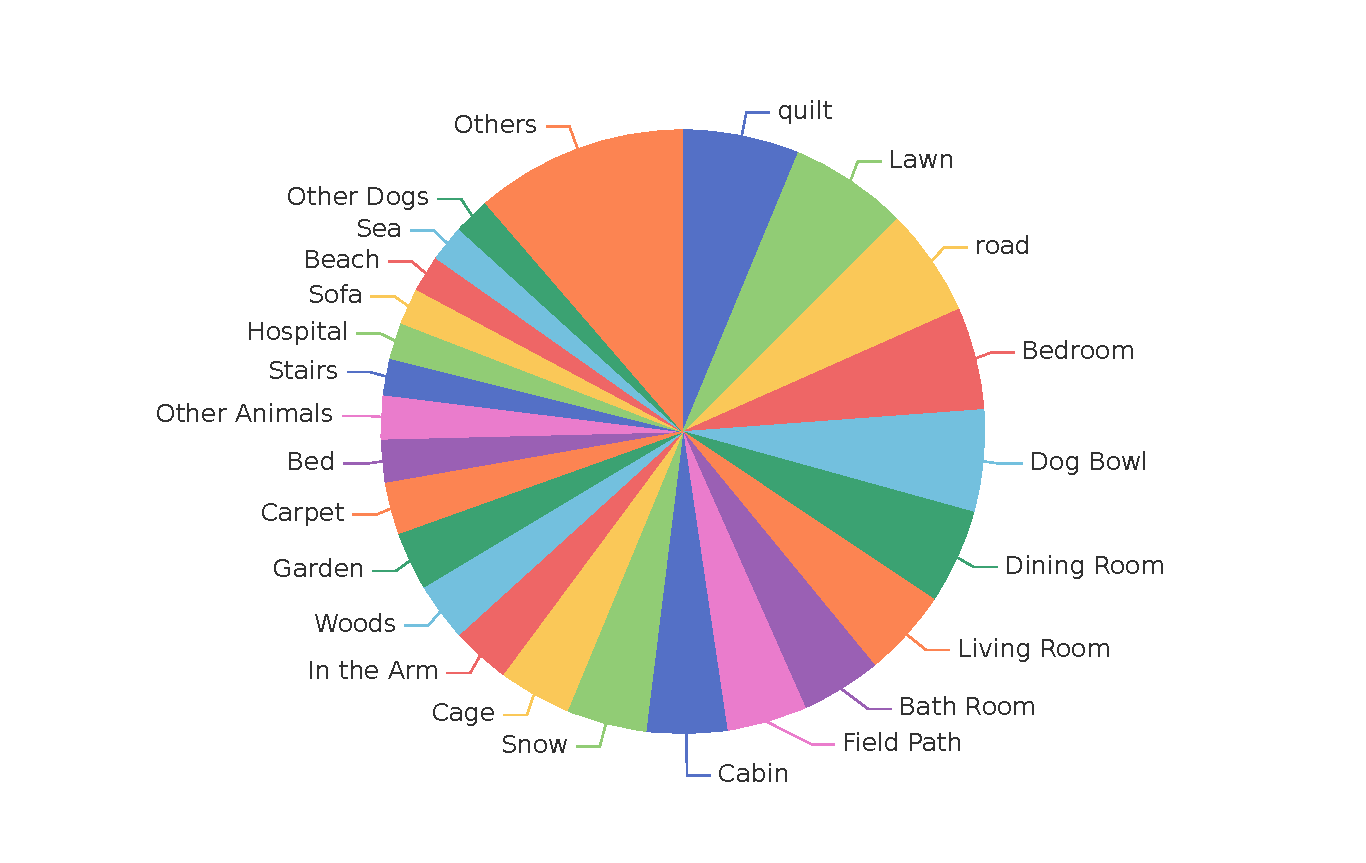
\includegraphics{total_scenes.pdf}}\\
(b) Scenes covered by ShibaScript. The scenes which occurrences is less than 1 were merged into ``others'', see~\secref{sec:appendix_a} for details.
\caption{The activities and scenes that covered by ShibaScript. The area of the patches represents the number of dogs producing this symbol.}
\label{fig:scene_and_activity}
\end{figure}

% \KZ{what do u mean by ``count''?} \MY{R u saying 16 = how many times? You can actually leave out the number here as the pie chart already suggests proportion info.}

% \begin{figure}[htbp]
        
% 	\centering
% 	\begin{subfigure}{0.24\linewidth}
% 		\centering
% 		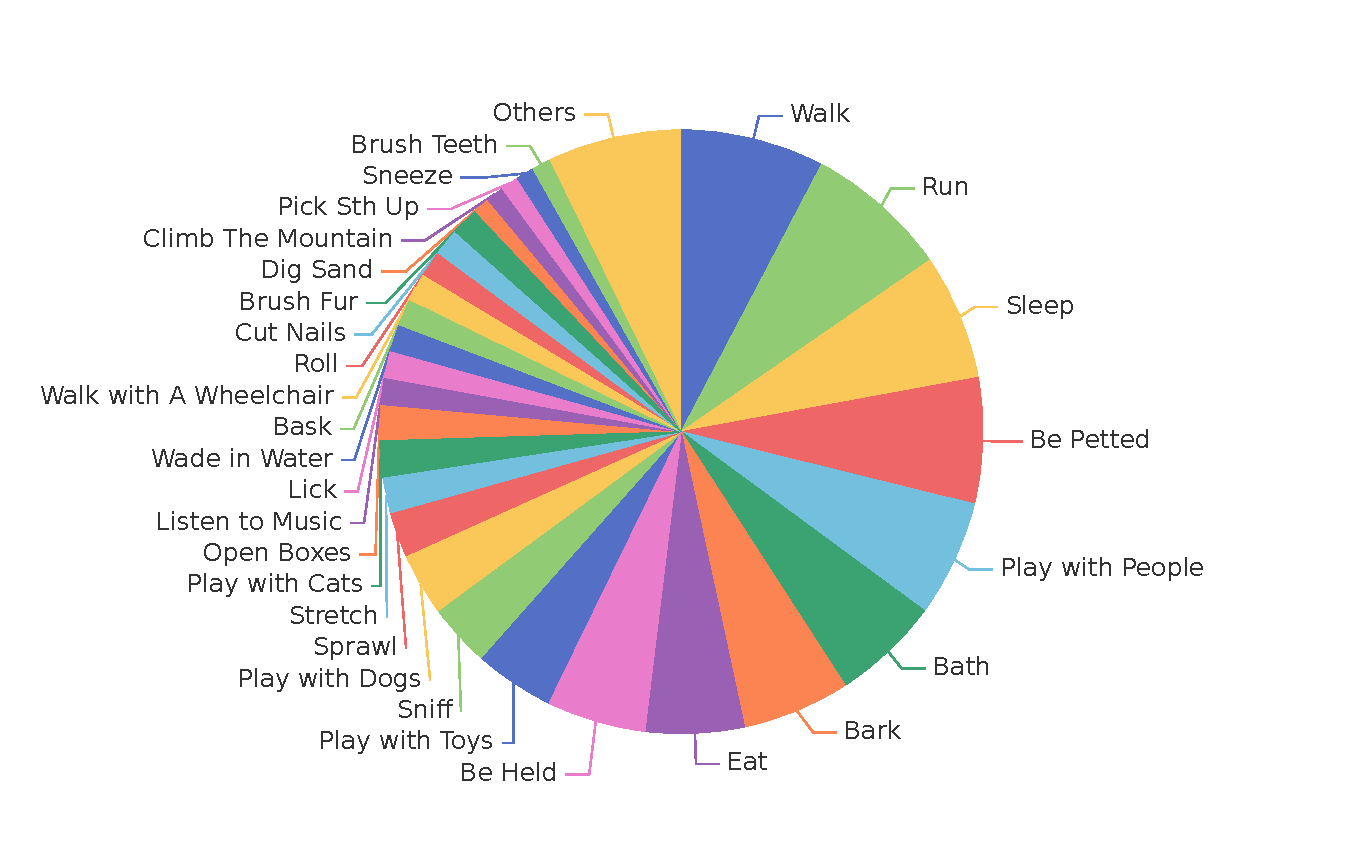
\includegraphics[width=0.9\linewidth]{total_activities.pdf}
% 		\caption*{Noisy}
% 	\end{subfigure}
% 	\centering
% 	\begin{subfigure}{0.24\linewidth}
% 		\centering
% 		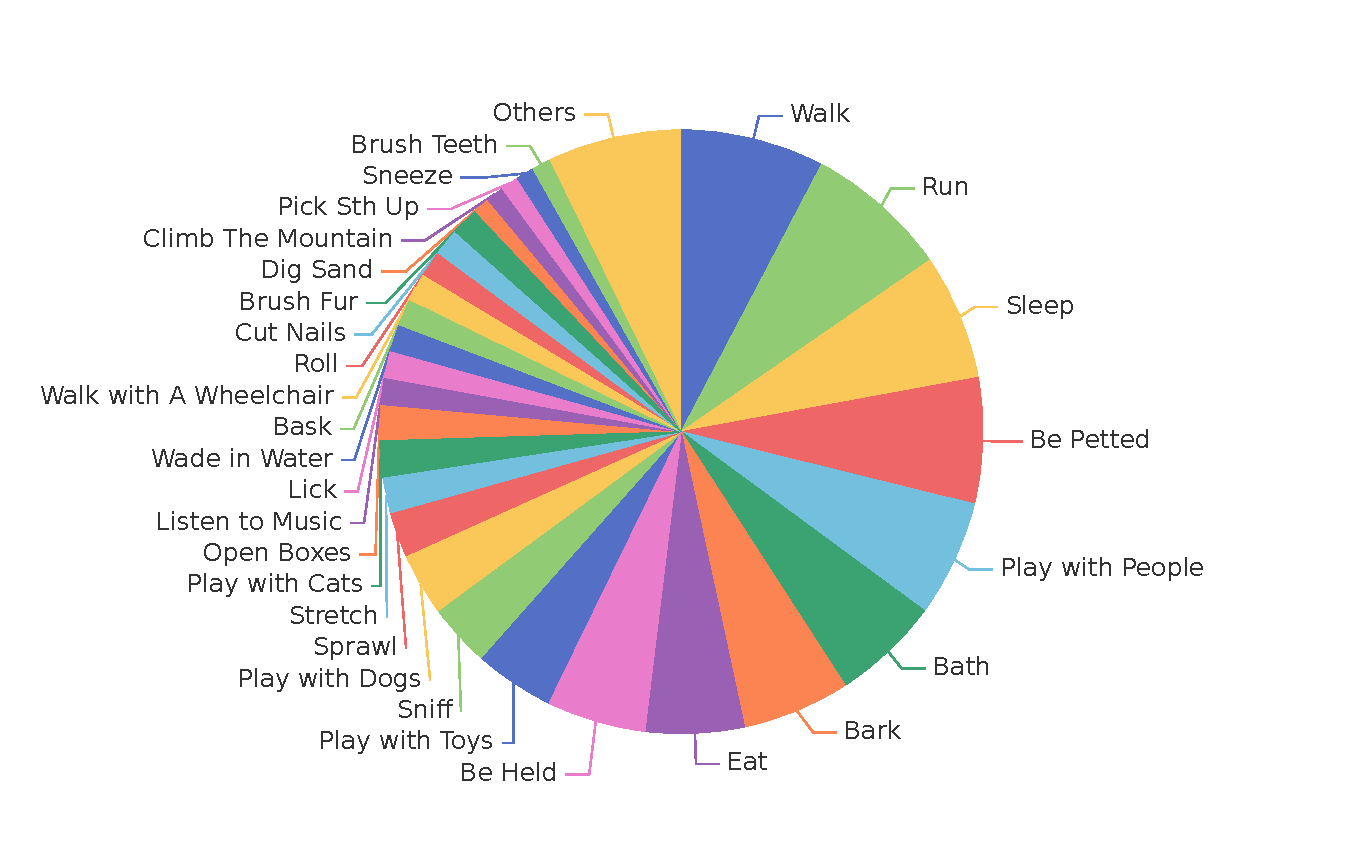
\includegraphics[width=0.9\linewidth]{total_activities.pdf}
% 		\caption*{Reference}
% 	\end{subfigure}
%         \caption{\CH{test subfig}}
%         \label{fig:visual_results}
% \end{figure}

% 多样性,不同的用户有不同的特定场景和活动,带来不常见的场景和活动,进一步提高数据集多样性,突出多来源的优点
Besides, there are some activities and scenes that appear rarely in the statistics. 
These activities and scenes are shown as ``others'' in~\figref{fig:scene_and_activity}. There are two possible reasons why an activity or scene appears infrequently. First of all, it is highly possible that this activity or scene is related to the personal characteristics of the user. For example, a dog has to wear a cone collar to prevent the dog from licking the wound, so the activity ``wear a cone collar'' appears only when the dog has had surgery, and this event is not a common one. The second reason is that users have different shooting habits, and a user may only record videos in certain scenes or activities. For example, some users only take indoor videos, so some outdoor activities and scenes like ``dig sand'' and ``beach'' are not possible to be covered in their videos, even if the dog actually participated in those activities or scenes. These activities and scenes with personal characteristics greatly expand the diversity of ShibaScript, so that it can cover some non-daily activities and scenes. Benefiting from the wide range of dogs, we can investigate a universal sound pattern of dogs, as they are extracted via them doing various activities under different scenes.

% \MY{You could add 1 or 2 sentences to talk about with this coverage, we can investigate a universal sound pattern of dogs, as they are extracted via them doing various activities under different scenes.}
% (TO APPENDIX)For activities, "others" includes "bow", "wag the tail", "pee", "die", "hum in the sleep", "dig the snow", "watch fireworks", "squat", "wear a muzzle", "wear a cone collar", "blow", "surf", "be vacuumed", "be medicated", "be brushed", "be massaged". For scenes, "others" includes "window", "fire", "shore", "heating pad", "hill", "stream", "vacuum", "under the bed", "cat tree", "shrine", "terrace", "bus", "mirror", "ice". 

 % \JY{Could you show the text-form result listing all the scenes and activities or give a picture to show that directly. I think only saying that will not make readers understand our statement.}
